\section{Synthesis}
\subsection{Resource Graph}
A resource graph is a graph $G_R = (V_R, E_R), V_R = V_S \cup V_T$, where
$V_S$ are the nodes from the sequence graph and $V_T$ are the different resource
types. It is bipartite, $E_R = V_S \times V_T, (v_s, v_t) \in E_R$ means $v_s$
can be executed on resource type $v_t$. Additionally there is a cost function
$c: V_T \to \mathbb{Z}$ and a execution time function $w: E_R \to \mathbb{Z}^{\geq 0}$

Furthermore $\alpha(v_t)$ denotes the number of available instances of resource
type $v_t$, $\beta(v_s)$ denotes on which resource type $v_s$ is running, and
$\gamma(v_s)$ denotes on which instance of this resource type it is running.

\subsection{Scheduling}
A schedule is a function $\tau: V_S \to \mathbb{Z}^{>0}$ that determines the
starting times of operations. It is feasible if
\begin{equation*}
	\forall (v_i, v_j) \in E_S . \tau(v_j) - \tau(v_i) \geq w(v_i)
\end{equation*}
where $w(v_i) = w(v_i, \beta(v_i))$ denotes the execution time of $v_i$.

The latency $L$ is $L = \tau(v_n) - \tau(v_0)$, the differnce between the
starting times.

\subsubsection{ASAP}
\begin{lstlisting}[escapeinside={(*}{*)}]
ASAP((*$V_S$*), (*$E_S$*), w) {
	\tau((*$v_0$*)) = 1
	do {
		(*$v_i \leftarrow \set{v \in V_S | \text{v's predecessors are planned}}$*);
		(*$\tau(v_i) = \max\set{\tau(v_j) + w(v_j) | (v_j, v_i) \in E_S}$*);
	} while (unplanned operations exist);
}
\end{lstlisting}

\subsection{ALAP}
\begin{lstlisting}[escapeinside={(*}{*)}]
ALAP((*$V_S$*), (*$E_S$*), w, (*$L_{max}$*)) {
	(*$\tau(v_n)$*) = (*$L_{max}$*) + 1;
	do {
		(*$v_i \leftarrow \set{v \in V_S | \text{v's successors are planned}}$*);
		(*$\tau(v_i) = \min\set{\tau(v_j) | (v_i, v_j) \in E_S} - w(v_i)$*);
	} while (unplanned operations exist);
}
\end{lstlisting}

\subsection{Bellman Ford}
One might add additional constraints as weighted edges in the sequence graph,
which can be resolved using Bellman Ford to find the single source longest path.
Set the weight of the normal edges to their execution times.

\begin{lstlisting}[escapeinside={(*}{*)}]
BELLMAN-FORD((*$V_S$*), (*$E_S$*), W) {
	(*$\tau_0^0$*) = 0;
	for (int i = 0; i < (*$\abs{V_S}$*); i++) (*$\tau_i^0 = w(v_0, v_i)$*);
	for (int j = 0; i < (*$\abs{V_S}$*); i++) {
		for (int i = 0; i < (*$\abs{V_S}$*); i++) {
			(*$\tau_i^{j+1}$*) = (*$\max\set{\tau_i^j, \tau_k^j + w(v_k, v_i) | k \neq i}$*);
		}
		if ((*$\forall i \,.\, \tau_i^{j+1} = \tau_i^j$*)) return true; // success
	}
	return false; // failed
}
\end{lstlisting}

\subsubsection{Example constraints}
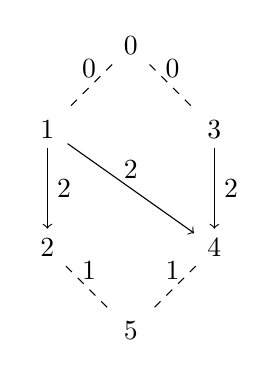
\begin{tikzpicture} [node distance=1.5cm]
	\tikzset{nop/.append style={minimum width=5mm}}
	\tikzset{inner/.append style={minimum width=5mm}}
	\node[nop]		(0)						{0};
	\node[inner]	(1) [below left of=0]	{1};
	\node[inner]	(2) [below of=1]		{2};
	\node[inner]	(3) [below right of=0]	{3};
	\node[inner]	(4)	[below of=3]		{4};
	\node[nop]		(5) [below right of=2]	{5};

	\path
		(0) edge[dashed]		node[above]	{0}		(1)
		(0) edge[dashed]		node[above]	{0}		(3)
		(1) edge[->]			node[right]	{2}		(2)
		(1) edge[->]			node[above]	{2}		(4)
		(3) edge[->]			node[right]	{2}		(4)
		(2) edge[dashed]		node[above]	{1}		(5)
		(4) edge[dashed]		node[above]	{1}		(5)
		;
\end{tikzpicture}

We add the following constraints
\begin{itemize}
	\item Between 1 and 2 there are at most 3 time units
	\item Between 0 and 4 there are at least 4 time units
\end{itemize}

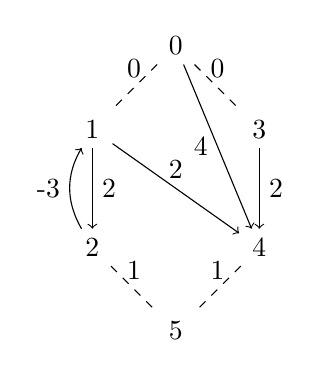
\begin{tikzpicture} [node distance=1.5cm]
	\tikzset{nop/.append style={minimum width=5mm}}
	\tikzset{inner/.append style={minimum width=5mm}}
	\node[nop]		(0)						{0};
	\node[inner]	(1) [below left of=0]	{1};
	\node[inner]	(2) [below of=1]		{2};
	\node[inner]	(3) [below right of=0]	{3};
	\node[inner]	(4)	[below of=3]		{4};
	\node[nop]		(5) [below right of=2]	{5};

	\path
		(0) edge[dashed]		node[above]	{0}		(1)
		(0) edge[dashed]		node[above]	{0}		(3)
		(1) edge[->]			node[right]	{2}		(2)
		(1) edge[->]			node[above]	{2}		(4)
		(3) edge[->]			node[right]	{2}		(4)
		(2) edge[dashed]		node[above]	{1}		(5)
		(4) edge[dashed]		node[above]	{1}		(5)
		(2) edge[bend left, ->]	node[left]	{-3}	(1)
		(0) edge[->]			node[left]	{4}		(4)
		;
\end{tikzpicture}

\subsection{List Scheduling}
\begin{lstlisting}[escapeinside={(*}{*)}]
LIST((*$V_S$*), (*$E_S$*), (*$V_R$*), (*$E_R$*), (*$\alpha$*), (*$\beta$*), priorities) {
	(*$V_T$*) = (*$V_R - V_S$*);
	t = 1;
	do {
		foreach((*$v_k \in V_T$*)) {
			(*$U_k$*) = candidates to be scheduled;
			(*$T_k$*) = running operations;
			(*$S_k$*) = subset of (*$U_k$*) with maximal priority and (*$\abs{S_k} + \abs{T_k} \leq \alpha(v_k)$*);
			foreach((*$v_i \in S_k$*)) { (*$\tau(v_i)$*) = t; }
		}
		t = t + 1;
	} while ((*$v_n$*) unplanned);
}
\end{lstlisting}

\subsection{Integer Linear Programming}
To get optimal results one can use ILP. First, for each $v_i \in V_S$ we have
to determine $l_i$ and $h_i$, the earliest and latest starting time
respectively, using ASAP and ALAP with a suitable $L_{max}$. $x_{i,t} = 1 \iff$
operation $v_i$ starts at time $t$.
\begin{align*}
	\min \tau(v_n) - \tau(v_0) &\qquad \text{subject to} \\
	\forall v_i \in V_S \forall l_i \leq t \leq h_i &\,.\,x_{i,t} \in \set{0, 1} \\
	\forall v_i \in V_S &\,.\, \sum_{t = l_i}^{h_i} x_{i,t} = 1 \\
	\forall v_i \in V_S &\,.\, \sum_{t = l_i}^{h_i} t \cdot x_{i,t} = \tau(v_i) \\
	\forall (v_i, v_j) \in E_S &\,.\, \tau(v_j) - \tau(v_i) \geq w(v_i) \\
	\forall v_k \in V_T \forall 1 \leq t \leq \max_i\set{h_i} &\,.\, \sum_{\forall i. (v_i, v_k) \in E_R} \sum_{p' = \max(0, t - h_i)}^{\min(w(v_i) - 1, t - l_i)} x_{i, t - p'} \leq \alpha(v_k)
\end{align*}

\subsubsection{Modifications}
To adapt the ILP to iterative algorithms (marked graphs, pipelining), replace
\begin{align*}
	\forall (v_i, v_j) \in E_S &\,.\, \tau(v_j) - \tau(v_i) \geq w(v_i) \\
	\forall v_k \in V_T \forall 1 \leq t \leq \max_i\set{h_i} &\,.\, \sum_{\forall i. (v_i, v_k) \in E_R} \sum_{p' = \max(0, t - h_i)}^{\min(w(v_i) - 1, t - l_i)} x_{i, t - p'} \leq \alpha(v_k)
\end{align*}
by
\begin{align*}
	\forall (v_i, v_j) \in E_S &\,.\, \tau(v_j) - \tau(v_i) \geq w(v_i) - d_{i,j} \cdot P\\
	\forall v_k \in V_T \forall 1 \leq t \leq \max_i\set{h_i} &\,.\, \sum_{\forall i. (v_i, v_k) \in E_R}
	\sum_{p' = 0}^{w(v_i) - 1} \sum_{\forall p \,.\, l_i \leq t - p' + p \cdot P \leq h_i} x_{i, t - p' + p \cdot P} \leq \alpha(v_k)
\end{align*}

and


where $d_{i,j}$ is the amount of tokens on edge $(i,j)$.

\subsection{DVS ILP}
\begin{align*}
	\min \sum_{k \in K} \sum_{v_i \in V_S} y_{ik} \cdot e_k(v_i) &\qquad\text{subject to} \\
	\forall v_i \in V_S, k \in K &\,.\, y_{ik} \in \set{0,1} \\
	\forall v_i \in V_S &\,.\, \sum_{k \in K} y_{ik} = 1 \\
	\forall (v_i, v_j) \in E_S &\,.\, \tau(v_j) - \tau(v_i) \geq \sum_{k \in K} y_{ik} \cdot w_k(v_i) \\
	\forall v_i \in V_S & \,.\, \tau(v_i) + \sum_{k \in K} y_{ik} \cdot w_k(v_i) \leq d(v_i)
\end{align*}
where $K$ is the set of voltage levels and there are no resource constraints.
